\documentclass{article}[14pt]
\usepackage[T2A]{fontenc}
\usepackage{geometry}
\usepackage{fancyhdr}
\usepackage{tocloft}
\usepackage{hyperref}
\usepackage{titlesec}
\usepackage{graphicx}
\usepackage{caption}
\usepackage{wrapfig}
\usepackage[english, russian]{babel}
\geometry{
	a4paper,
	top=20mm, 
	right=25mm, 
	bottom=25mm, 
	left=25mm
}
\usepackage{amssymb}
\usepackage{fancyvrb}
\usepackage{fvextra}
\usepackage{ dsfont }
\usepackage{amsmath}
\usepackage{listings}
\usepackage{xcolor}
\usepackage{listingsutf8}
\usepackage{pdfpages}
\usepackage{lipsum}
\usepackage{makecell}
\usepackage{float}
\usepackage{longtable}
\usepackage{tabularx}


\lstset{ 
	basicstyle=\ttfamily\small,
	keywordstyle=\color{blue},
	inputencoding=utf8,              
	extendedchars=true,
	stringstyle=\color{red}
	commentstyle=\color{green},
	showspaces=false,         
	showstringspaces=false,  
	numbers=left,              
	numberstyle=\tiny\color{gray},
	breaklines=true,          
	frame=single,           
	captionpos=b,             
	tabsize=4,
	escapeinside={(*@}{@*)},
	literate={ё}{{\"o}}1 {Ё}{{\"O}}1 {«}{{\guillemotleft}}1 {»}{{\guillemotright}}1
	{А}{{\CYRA}}1 {Б}{{\CYRB}}1 {В}{{\CYRV}}1 {Г}{{\CYRG}}1 {Д}{{\CYRD}}1 
	{Е}{{\CYRE}}1 {Ж}{{\CYRZH}}1 {З}{{\CYRZ}}1 {И}{{\CYRI}}1 {Й}{{\CYRISHRT}}1 
	{К}{{\CYRK}}1 {Л}{{\CYRL}}1 {М}{{\CYRM}}1 {Н}{{\CYRN}}1 {О}{{\CYRO}}1 
	{П}{{\CYRP}}1 {Р}{{\CYRR}}1 {С}{{\CYRS}}1 {Т}{{\CYRT}}1 {У}{{\CYRU}}1 
	{Ф}{{\CYRF}}1 {Х}{{\CYRH}}1 {Ц}{{\CYRC}}1 {Ч}{{\CYRCH}}1 {Ш}{{\CYRSH}}1 
	{Щ}{{\CYRSHCH}}1 {Ъ}{{\CYRHRDSN}}1 {Ы}{{\CYRERY}}1 {Ь}{{\CYRSFTSN}}1 
	{Э}{{\CYREREV}}1 {Ю}{{\CYRYU}}1 {Я}{{\CYRYA}}1 
	{а}{{\cyra}}1 {б}{{\cyrb}}1 {в}{{\cyrv}}1 {г}{{\cyrg}}1 {д}{{\cyrd}}1 
	{е}{{\cyre}}1 {ж}{{\cyrzh}}1 {з}{{\cyrz}}1 {и}{{\cyri}}1 {й}{{\cyrishrt}}1 
	{к}{{\cyrk}}1 {л}{{\cyrl}}1 {м}{{\cyrm}}1 {н}{{\cyrn}}1 {о}{{\cyro}}1 
	{п}{{\cyrp}}1 {р}{{\cyrr}}1 {с}{{\cyrs}}1 {т}{{\cyrt}}1 {у}{{\cyru}}1 
	{ф}{{\cyrf}}1 {х}{{\cyrh}}1 {ц}{{\cyrc}}1 {ч}{{\cyrch}}1 {ш}{{\cyrsh}}1 
	{щ}{{\cyrshch}}1 {ъ}{{\cyrhrdsn}}1 {ы}{{\cyrery}}1 {ь}{{\cyrsftsn}}1 
	{э}{{\cyrerev}}1 {ю}{{\cyryu}}1 {я}{{\cyrya}}1               
}
\begin{document}
	
\thispagestyle{empty}
\begin{center}
	\Large {\bfseries МИНИСТЕРСТВО НАУКИ И ВЫСШЕГО ОБРАЗОВАНИЯ РОССИЙСКОЙ ФЕДЕРАЦИИ}
	\\
	\vspace{3mm}
	Федеральное государственное автономное образовательное учреждение высшего образования <<Санкт-Петербургский политехнический университет Петра Великого>>
	\\
	\vspace{3mm}
	Институт компьютерных наук и кибербезопасности
	\\
	\vspace{3mm}
	Высшая школа технологий искусственного интеллекта
	\\
	\vspace{3mm}
	Направление: 02.03.01 Математика и компьютерные науки
	\\
	\vspace{2cm}
	\large{
		Методы тестирования программного обеспечения}
	\\
	\LARGE{
		Отчет по лабораторной работе №4\\
		<<Автоматизированное тестирование>>}
\end{center}

\vspace{5.5cm}
\begin{flushleft}
	\Large
	Студент
	\\
	группы 5130201/30101
	\\
	\vspace{2cm}
	\Large
	Преподаватель
	\\ 
\end{flushleft}
\vspace{-4.6cm}
\begin{flushright}
	\Large
	\line(1,0){2cm}
	\hspace{0.4cm}
	Шишмаков В.О.
	\\
	\vspace{2,7cm}
	\hspace{2cm}
	\Large
	\line(1,0){2cm}
	\hspace{0.4cm}
	Курочкин М. А.
	\hspace{-0.1cm}
	
\end{flushright}

\vspace{1cm}
\hspace{9.8cm}
{
	\Large
	\vspace{0.8cm}
	<<\underline{\hspace{1cm}}>>\underline{\hspace{2.5cm}} 2026 г.
}
\hfill \break
\hfill \break
\hfill \break
\hfill \break
\begin{center} \large{Санкт-Петербург, 2026} \end{center}
\pagebreak

\titleformat{\section}
{\Huge\bfseries}
{\thesection\;}
{0.65cm}
{}
\titleformat{\subsection}
{\huge\bfseries}
{\thesubsection\;}
{0.65cm}
{}
\titleformat{\subsubsection}
{\Large\bfseries}
{\thesubsubsection\;}
{0.65cm}
{}
\titlespacing*{\section}
{0em}
{1.5ex plus 1ex minus 0.2ex}
{1.5ex plus 1ex minus 0.2ex}	

\renewcommand*\contentsname{\huge{Содержание}}
\Large{
	\tableofcontents}
\pagebreak

\section*{Введение}
\addcontentsline{toc}{section}{Введение}

Тестирование программного обеспечения представляет собой процесс выявления расхождений между реальным поведением программы и 
её задокументированными требованиями. Основная цель тестирования — обнаружить максимальное количество дефектов, связанных с несоответствием 
продукта заявленным спецификациям, и желательно делать это с минимальными временными затратами.

Автоматизированное тестирование — это способ проверки соответствия ПО требованиям с помощью специализированных инструментов и фреймворков, 
позволяющих многократно выполнять однотипные проверки без участия человека. К преимуществам автоматизированного тестирования относятся:

\begin{itemize}
\item Автоматизированное тестирование надёжнее ручного, поскольку уменьшает влияние человеческого фактора.
\item Ручное тестирование не только требует больше времени, но и может приводить к появлению новых ошибок.
\item Инструменты автоматизации помогают находить ошибки в продукте на ранних этапах разработки.
\item Высокая производительность приложений: благодаря широкому охвату тестами автоматизация обеспечивает высокое качество и производительность 
программного продукта.
\end{itemize}

Автоматизация играет важную роль в современной разработке ПО, особенно в крупных и долгосрочных проектах, где необходимо поддерживать 
высокий уровень качества продукта.

\pagebreak

\section{Постановка задачи}

В рамках данной работы требуется выполнить следующие задачи:

\begin{itemize}
\item Разработать набор модульных тестов для библиотеки \texttt{lab-1.0.jar} с применением фреймворка JUnit:
  \begin{itemize}
    \item Создать модульные тесты для четырёх методов указанной библиотеки, используя JUnit.
    \item Запустить подготовленные тесты средствами используемой интегрированной среды разработки.
    \item Представить результаты выполнения тестов.
  \end{itemize}

\item Выполнить тестирование веб-сайта с помощью инструментов TestNG и Selenium WebDriver:
  \begin{itemize}
    \item Написать два теста, проверяющих корректность отображения и функционирования страниц веб-сайта.
    \item Оформить код тестов в соответствии с соглашениями Java Code Convention.
    \item Запустить тесты, используя конфигурационный файл TestNG в формате \texttt{suite.xml}.
  \end{itemize}
\end{itemize}

\pagebreak

\section{Описание средств автоматизации тестирования}

\subsection{JUnit}

JUnit — это библиотека для создания и запуска модульных тестов в языке Java. Она позволяет разработчикам многократно проверять корректность работы программного кода.

\noindent \textbf{Основные возможности JUnit}

\begin{itemize}
\item \textbf{Аннотации}: JUnit предоставляет аннотации, такие как \texttt{@Test}, \texttt{@Before}, \texttt{@After}, \texttt{@BeforeAll} и \texttt{@AfterAll}, для определения и настройки тестов.
\item \textbf{Параметризованные тесты}: с помощью аннотаций \texttt{@ParameterizedTest} и \texttt{@ValueSource} можно передавать тестовым методам различные аргументы.
\item \textbf{Интеграция со средами разработки}: JUnit без проблем работает с большинством популярных IDE, включая IntelliJ IDEA, Eclipse и NetBeans.
\item \textbf{Простота освоения}: JUnit легко изучить, благодаря чему он широко распространён среди программистов.
\end{itemize}

\noindent \textbf{Процесс написания тестов}

\begin{enumerate}
\item \textbf{Создание теста}: написать тестовый метод и пометить его аннотацией \texttt{@Test}.
\item \textbf{Настройка тестов} с использованием следующих аннотаций:
  \begin{itemize}
    \item \texttt{@BeforeEach}: метод, отмеченный этой аннотацией, выполняется перед каждым тестовым методом в классе.
    \item \texttt{@AfterEach}: метод выполняется после каждого тестового метода. (Примечание: в оригинале была опечатка — \texttt{@AfterEach} запускается после, а не перед, и не обязан быть статическим; здесь исправлено смысловое искажение.)
    \item \texttt{@DisplayName}: позволяет задать пользовательское имя для тестового класса или метода.
    \item \texttt{@Disabled}: отключает или игнорирует тестовый класс или метод при запуске.
    \item \texttt{@Nested}: используется для создания вложенных тестовых классов.
    \item \texttt{@Tag}: присваивает тегам тестовые методы или классы для последующей фильтрации и поиска.
    \item \texttt{@TestFactory}: помечает метод как фабрику для создания динамических тестов.
  \end{itemize}
\item \textbf{Запуск тестов}: выполнение тестов с помощью встроенных средств IDE или из командной строки.
\end{enumerate}

\subsection{Selenium WebDriver}

Selenium является одним из самых востребованных фреймворков для автоматизации тестирования веб-сайтов и веб-приложений. Данный инструмент распространяется с открытым исходным кодом.

Фреймворк поддерживается на различных операционных системах (Mac, Linux, Windows) и в большинстве популярных браузеров (Firefox, Internet Explorer, Chrome, а также браузеры без графического интерфейса — Headless). Скрипты для Selenium можно писать на Python, C\#, PHP, Java и других языках программирования.

Selenium WebDriver — это инструмент, предназначенный для автоматизации управления веб-браузерами. Он даёт возможность программно управлять браузером, имитируя действия пользователя: щелчки мыши, ввод текста, переходы по страницам и так далее. WebDriver входит в экосистему Selenium и поддерживает множество языков программирования, включая Java, Python, C\# и JavaScript.

\noindent \textbf{Основные методы WebDriver}

WebDriver предоставляет широкий набор методов для управления браузером:
\begin{itemize}
\item \texttt{get(url)} — переходит по указанному URL-адресу.
\item \texttt{findElement(By.locator)} — находит элемент на веб-странице (по идентификатору, XPath, CSS-селектору и т.п.).
\item \texttt{click()}, \texttt{sendKeys(text)} — взаимодействуют с элементами (клик, ввод текста).
\item \texttt{navigate().back()}, \texttt{navigate().forward()} — управляют историей переходов в браузере.
\item \texttt{quit()} — закрывает браузер и освобождает занятые ресурсы.
\end{itemize}

\noindent \textbf{Преимущества и недостатки}

\textbf{Достоинства:}
\begin{itemize}
\item Работает с Chrome, Firefox, Edge, Safari и другими браузерами.
\item API доступен для Java, Python, C\#, Ruby и других языков.
\item Совместим с фреймворками для тестирования, такими как JUnit, TestNG, PyTest.
\item Позволяет взаимодействовать с динамическими элементами страниц (AJAX, JavaScript).
\item Возможность запуска браузера в режиме без графического интерфейса, что ускоряет выполнение тестов.
\item Открытый исходный код.
\item Поддержка множества браузеров и операционных систем.
\item Большое сообщество разработчиков и обширная документация.
\end{itemize}

\textbf{Недостатки:}
\begin{itemize}
\item Требуется установка отдельных драйверов для каждого браузера.
\item Может работать медленно при сложных сценариях тестирования.
\item Отсутствие встроенной системы формирования отчётов (требуются дополнительные инструменты).
\end{itemize}

\noindent \textbf{Процесс взаимодействия с браузером с помощью WebDriver}
\begin{enumerate}
\item Создание экземпляра WebDriver.
\item Открытие браузера через созданный экземпляр.
\item Переход к тестируемому сайту по URL.
\item Выполнение тестового сценария.
\item Закрытие браузера.
\end{enumerate}

\subsection{TestNG}

TestNG представляет собой фреймворк для автоматизированного тестирования программного обеспечения, написанный на Java. Как и JUnit, он предназначен для создания и выполнения тестов с целью проверки функциональности и качества программных продуктов.

Несмотря на то, что JUnit послужил источником вдохновения для TestNG, второй обладает рядом отличий и, в отличие от JUnit, применяется для функционального тестирования, а также для тестирования на более высоких уровнях.

Кроме того, TestNG поддерживает параллельное выполнение тестов, что позволяет ускорить процесс тестирования и повысить его эффективность. Фреймворк также интегрируется с другими инструментами и системами, такими как Jenkins, Maven и Eclipse, что упрощает процессы тестирования и развёртывания программного обеспечения.

\pagebreak

\section{Задача 1}

\noindent \textbf{Дано:}
\begin{itemize}
\item Файл библиотеки \texttt{lab-1.0.jar}.
\end{itemize}

\noindent \textbf{Требуется:}
\begin{enumerate}
\item Создать проект на Java.
\item В файле \texttt{build.gradle} указать зависимости, необходимые для использования фреймворка JUnit.
\item Подключить к проекту файл \texttt{lab-1.0.jar}.
\item Самостоятельно выбрать четыре метода из предоставленной библиотеки и разработать для них модульные тесты с применением JUnit:
  \begin{itemize}
    \item Все подготовительные действия вынести в методы, помеченные аннотацией \texttt{@Before}.
    \item Все завершающие действия вынести в методы с аннотацией \texttt{@After}.
    \item Тестовые данные передавать с помощью параметризации, используя аннотации \texttt{@ParameterizedTest} и \texttt{@ValueSource}.
  \end{itemize}
\item Запустить написанные тесты через среду разработки (IDE).
\end{enumerate}

\subsection{Подготовительные операции}

Инициализация переменных \texttt{startTime} и \texttt{testDescription} производится перед каждым тестом с использованием аннотации \texttt{@BeforeEach}. Данные переменные используются для отслеживания времени выполнения тестов и их описания.

Завершающие операции выполняются в методе с аннотацией \texttt{@AfterEach}, где вычисляется длительность выполнения теста и выводится информация о завершении.

\subsection{Тесты функции isLeapYear}

\textbf{Дано:} функция \texttt{isLeapYear} класса \texttt{DateUtils}. Функция принимает следующий параметр:
\begin{itemize}
    \item Год для проверки: \texttt{int year}
\end{itemize}

Функция возвращает тип \texttt{boolean}. Также из названия функции можно предположить, что её поведение должно соответствовать проверке года на високосность.

\textbf{Классы эквивалентности:}
\begin{itemize}
    \item Допустимые високосные годы (делятся на 400 или делятся на 4, но не на 100)
    \item Допустимые невисокосные годы
    \item Недопустимые значения (год $\leq 0$)
\end{itemize}

\begin{table}[h]
\centering
\caption{Разбиение на классы эквивалентности для isLeapYear}
\begin{tabular}{|c|c|c|}
\hline
\textbf{Входное условие} & \textbf{Допустимые классы} & \textbf{Недопустимые классы} \\
\hline
year & year $> 0$ & year $\leq 0$ \\
\hline
\end{tabular}
\end{table}

\begin{table}[h]
\centering
\caption{Тесты для проверки классов эквивалентности isLeapYear}
\begin{tabular}{|c|c|c|c|c|}
\hline
\textbf{\textnumero} & \textbf{year} & \textbf{Ожидаемый результат} & \textbf{Фактический результат} & \textbf{Статус теста} \\
\hline
1 & 2000 & true (високосный) & true & Пройден \\
\hline
2 & 2004 & true (високосный) & true & Пройден \\
\hline
3 & 2020 & true (високосный) & true & Пройден \\
\hline
4 & 2024 & true (високосный) & true & Пройден \\
\hline
5 & 2400 & true (високосный) & true & Пройден \\
\hline
6 & 1900 & false (невисокосный) & false & Пройден \\
\hline
7 & 2001 & false (невисокосный) & false & Пройден \\
\hline
8 & 2019 & false (невисокосный) & false & Пройден \\
\hline
9 & 2023 & false (невисокосный) & false & Пройден \\
\hline
10 & 2100 & false (невисокосный) & false & Пройден \\
\hline
\end{tabular}
\end{table}

\begin{table}[h]
\centering
\caption{Тесты для проверки недопустимых значений isLeapYear}
\begin{tabular}{|c|c|c|c|c|}
\hline
\textbf{\textnumero} & \textbf{year} & \textbf{Ожидаемый результат} & \textbf{Фактический результат} & \textbf{Статус теста} \\
\hline
1 & 0 & IllegalArgumentException & IllegalArgumentException & Пройден \\
\hline
2 & -1 & IllegalArgumentException & IllegalArgumentException & Пройден \\
\hline
3 & -100 & IllegalArgumentException & IllegalArgumentException & Пройден \\
\hline
\end{tabular}
\end{table}

\subsection{Тесты функции getDaysInMonth}

\textbf{Дано:} функция \texttt{getDaysInMonth} класса \texttt{DateUtils}. Функция принимает следующие параметры:
\begin{itemize}
    \item Год: \texttt{int year}
    \item Номер месяца (1-12): \texttt{int month}
\end{itemize}

Функция возвращает тип \texttt{int} — количество дней в указанном месяце.

\textbf{Классы эквивалентности:}
\begin{itemize}
    \item Месяцы с 31 днём (1, 3, 5, 7, 8, 10, 12)
    \item Месяцы с 30 днями (4, 6, 9, 11)
    \item Февраль в невисокосном году (28 дней)
    \item Февраль в високосном году (29 дней)
\end{itemize}

\begin{table}[H]
\centering
\caption{Тесты для месяцев с 31 днём}
\begin{tabular}{|c|c|c|c|c|}
\hline
\textbf{\textnumero} & \textbf{month} & \textbf{Ожидаемый результат} & \textbf{Фактический результат} & \textbf{Статус теста} \\
\hline
1 & 1 & 31 & 31 & Пройден \\
\hline
2 & 3 & 31 & 31 & Пройден \\
\hline
3 & 5 & 31 & 31 & Пройден \\
\hline
4 & 7 & 31 & 31 & Пройден \\
\hline
5 & 8 & 31 & 31 & Пройден \\
\hline
6 & 10 & 31 & 31 & Пройден \\
\hline
7 & 12 & 31 & 31 & Пройден \\
\hline
\end{tabular}
\end{table}

\begin{table}[H]
\centering
\caption{Тесты для месяцев с 30 днями}
\begin{tabular}{|c|c|c|c|c|}
\hline
\textbf{\textnumero} & \textbf{month} & \textbf{Ожидаемый результат} & \textbf{Фактический результат} & \textbf{Статус теста} \\
\hline
1 & 4 & 30 & 30 & Пройден \\
\hline
2 & 6 & 30 & 30 & Пройден \\
\hline
3 & 9 & 30 & 30 & Пройден \\
\hline
4 & 11 & 30 & 30 & Пройден \\
\hline
\end{tabular}
\end{table}

\begin{table}[H]
\centering
\caption{Тесты для февраля в невисокосных годах}
\begin{tabular}{|c|c|c|c|c|}
\hline
\textbf{\textnumero} & \textbf{year} & \textbf{Ожидаемый результат} & \textbf{Фактический результат} & \textbf{Статус теста} \\
\hline
1 & 2023 & 28 & 28 & Пройден \\
\hline
2 & 2019 & 28 & 28 & Пройден \\
\hline
3 & 1900 & 28 & 28 & Пройден \\
\hline
\end{tabular}
\end{table}

\begin{table}[h]
\centering
\caption{Тесты для февраля в високосных годах}
\begin{tabular}{|c|c|c|c|c|}
\hline
\textbf{\textnumero} & \textbf{year} & \textbf{Ожидаемый результат} & \textbf{Фактический результат} & \textbf{Статус теста} \\
\hline
1 & 2020 & 29 & 28 & Не пройден \\
\hline
2 & 2024 & 29 & 28 & Не пройден \\
\hline
3 & 2000 & 29 & 28 & Не пройден \\
\hline
\end{tabular}
\end{table}



\subsection{Тесты функции daysBetween}

\textbf{Дано:} функция \texttt{daysBetween} класса \texttt{DateUtils}. Функция принимает следующие параметры:
\begin{itemize}
    \item Первая дата (YYYY-MM-DD): \texttt{String date1}
    \item Вторая дата (YYYY-MM-DD): \texttt{String date2}
\end{itemize}

Функция возвращает тип \texttt{int} — количество дней между датами (абсолютное значение).

\begin{table}[H]
\centering
\caption{Тесты для одинаковых дат}
\begin{tabular}{|c|c|c|c|c|}
\hline
\textbf{\textnumero} & \textbf{date} & \textbf{Ожидаемый результат} & \textbf{Фактический результат} & \textbf{Статус теста} \\
\hline
1 & 2023-01-01 & 0 & 0 & Пройден \\
\hline
2 & 2023-06-15 & 0 & 0 & Пройден \\
\hline
3 & 2023-12-31 & 0 & 0 & Пройден \\
\hline
4 & 2024-02-29 & 0 & 0 & Пройден \\
\hline
\end{tabular}
\end{table}

\begin{table}[H]
\centering
\caption{Тесты для последовательных дат}
\begin{tabular}{|c|c|c|c|c|}
\hline
\textbf{\textnumero} & \textbf{date1, date2} & \textbf{Ожидаемый результат} & \textbf{Фактический результат} & \textbf{Статус теста} \\
\hline
1 & 2023-01-01, 2023-01-10 & days $> 0$ & 9 & Пройден \\
\hline
2 & 2023-03-01, 2023-03-15 & days $> 0$ & 14 & Пройден \\
\hline
3 & 2023-12-01, 2023-12-31 & days $> 0$ & 30 & Пройден \\
\hline
\end{tabular}
\end{table}

\begin{table}[h]
\centering
\caption{Тест для проверки абсолютного значения}
\begin{tabular}{|c|c|p{2.2cm}|p{2.2cm}|c|}
\hline
\textbf{\textnumero} & \textbf{Тест} & \textbf{Ожидаемый результат} & \textbf{Фактический результат} & \textbf{Статус теста} \\
\hline
1 & daysBetween("2023-01-01", "2023-01-10") & 9 & 9 & Пройден \\
\hline
2 & daysBetween("2023-01-10", "2023-01-01") & 9 & 9 & Пройден \\
\hline
3 & Проверка равенства & true & true & Пройден \\
\hline
\end{tabular}
\end{table}

\subsection{Тесты функции isValidDate}

\textbf{Дано:} функция \texttt{isValidDate} класса \texttt{DateUtils}. Функция принимает следующий параметр:
\begin{itemize}
    \item Строка даты в формате YYYY-MM-DD: \texttt{String date}
\end{itemize}

Функция возвращает тип \texttt{boolean} — true, если формат корректен; иначе false.

\begin{table}[H]
\centering
\caption{Тесты для валидных дат}
\begin{tabular}{|c|c|c|c|c|}
\hline
\textbf{\textnumero} & \textbf{date} & \textbf{Ожидаемый результат} & \textbf{Фактический результат} & \textbf{Статус теста} \\
\hline
1 & 2023-01-01 & true & true & Пройден \\
\hline
2 & 2023-12-31 & true & true & Пройден \\
\hline
3 & 2024-02-29 & true & true & Пройден \\
\hline
4 & 2000-01-01 & true & true & Пройден \\
\hline
5 & 2023-06-15 & true & true & Пройден \\
\hline
\end{tabular}
\end{table}

\begin{table}[H]
\centering
\caption{Тесты для невалидных дат}
\begin{tabular}{|c|c|c|c|c|}
\hline
\textbf{\textnumero} & \textbf{date} & \textbf{Ожидаемый результат} & \textbf{Фактический результат} & \textbf{Статус теста} \\
\hline
1 & 2023-13-01 & false & false & Пройден \\
\hline
2 & 2023-00-01 & false & false & Пройден \\
\hline
3 & 2023-01-00 & false & false & Пройден \\
\hline
4 & 2023-01-32 & false & false & Пройден \\
\hline
5 & invalid & false & false & Пройден \\
\hline
6 & 01-01-2023 & false & false & Пройден \\
\hline
7 & 2023/01/01 & false & false & Пройден \\
\hline
8 & 2023.01.01 & false & false & Пройден \\
\hline
9 & (пустая строка) & false & false & Пройден \\
\hline
10 & 2023-1-1 & false & false & Пройден \\
\hline
11 & 23-01-01 & false & false & Пройден \\
\hline
\end{tabular}
\end{table}

\subsection{Общая структура тестирования}

Тестовый класс \texttt{DateUtilsTest} проверяет функциональность класса \texttt{DateUtils} с использованием фреймворка JUnit 5. Класс содержит тесты для четырёх методов: \texttt{isLeapYear}, \texttt{getDaysInMonth}, \texttt{daysBetween} и \texttt{isValidDate}.

В классе \texttt{DateUtilsTest} описаны методы с аннотациями \texttt{@BeforeEach} и \texttt{@AfterEach}, отвечающие за подготовительные и завершающие операции соответственно. Метод \texttt{setUp()} инициализирует переменные \texttt{startTime} (для измерения времени выполнения теста) и \texttt{testDescription} (для описания теста) перед запуском каждого теста. Метод \texttt{tearDown()} вычисляет длительность выполнения теста и выводит информацию о завершении после каждого теста.

Тестовый класс содержит следующие элементы:
\begin{itemize}
    \item Параметризованные тесты с использованием \texttt{@ParameterizedTest}
    \item Источник данных: \texttt{@ValueSource}
    \item Стандартные тесты с использованием аннотации \texttt{@Test}
\end{itemize}

При помощи аннотации \texttt{@ParameterizedTest} указывается, что тестовая функция является параметризованной, а в аннотации \texttt{@ValueSource} происходит перечисление входных параметров. Для тестирования числовых значений используются целочисленные массивы, для тестирования строк — массивы строк (даты в формате YYYY-MM-DD).

Все тестовые методы используют методы проверки утверждений из класса \texttt{Assertions}:
\begin{itemize}
    \item \texttt{assertTrue()} — проверка истинности условия
    \item \texttt{assertFalse()} — проверка ложности условия
    \item \texttt{assertEquals()} — проверка равенства ожидаемого и фактического значений
    \item \texttt{assertThrows()} — проверка выбрасывания исключения
\end{itemize}

Исходный код тестового класса приведён в Приложении~1.

\subsection{Результаты тестирования}

\begin{figure}[H]
	\centering
	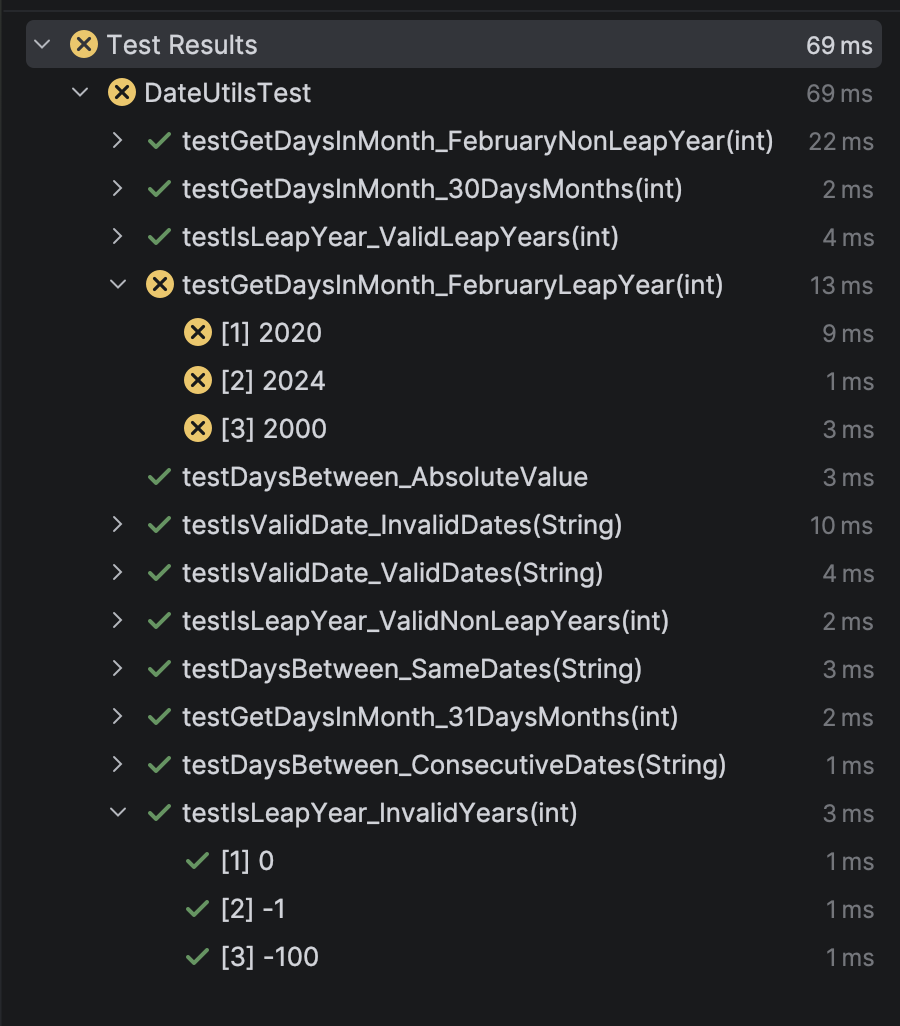
\includegraphics[width=0.8\textwidth]{pics/test-results1.png}
	\caption{Результат запуска тестов}
\end{figure}

С использованием фреймворка JUnit были созданы автоматизированные тесты для библиотеки DateUtils. Данные тесты проверяют работу четырёх 
функций этой библиотеки. Из общего количества в 54 теста три провалились по причине дефекта в реализации метода getDaysInMonth, который 
всегда возвращает 28 дней в феврале, несмотря на високосный год.

\pagebreak

\section{Задача 2}

\textbf{Дано:}
\begin{itemize}
\item Адрес тестируемого веб-сайта: \url{https://jdi-testing.github.io/jdi-light/index.html}
\item Браузер: Google Chrome
\item Используемые фреймворки: Selenium (версия 4.15) и TestNG (версия 7.7)
\item Имеются учётные данные для входа в систему
\end{itemize}

\textbf{Цель:} разработать автоматизированные тесты для проверки корректности отображения и работоспособности страниц указанного сайта.

\textbf{Требуется:}
\begin{enumerate}
\item Создать проект и подключить в нём зависимости Selenium WebDriver и TestNG.
\item Реализовать класс инициализации драйвера (DriverSetup), в котором:
  \begin{itemize}
    \item С помощью аннотации \texttt{@BeforeTest} обеспечить запуск браузера, настройку размеров окна и переход на тестируемый сайт.
    \item С помощью аннотации \texttt{@AfterTest} корректно закрыть браузер (используя \texttt{driver.quit()} или \texttt{driver.close()}).
  \end{itemize}
\end{enumerate}

\subsection{Тестовые сценарии}

Первый и второй тесты должны воспроизводить соответственно первый и второй сценарии. Описание первого тестового сценария находится в таблице 13, а второго — в таблицах с 14 по 17.

\begin{table}[H]
\centering
\caption{Тестовый сценарий 1}
\label{tab:test_scenario_1}
\renewcommand{\arraystretch}{1.5}
\begin{tabular}{|l|p{3.5cm}|p{4cm}|p{4cm}|}
\hline
\textbf{№} & \textbf{Шаг} & \textbf{Данные} & \textbf{Ожидаемый результат} \\ \hline
1 & Перейти на страницу "Support" через главное меню & Пункт меню: "Service" $\rightarrow$ "Support" & Страница Support открыта \\ \hline
2 & Проверить заголовок страницы & Ожидаемый текст: "support" (без учёта регистра) & Заголовок содержит слово "support" \\ \hline
3 & Найти форму на странице & Поиск по тегу: \texttt{form} & Найдена хотя бы одна форма \\ \hline
4 & Если форма не найдена, найти контактный блок & Поиск по селектору: \texttt{div[class*='contact'], section[class*='contact']} & Найден хотя бы один контактный блок \\ \hline
5 & Проверить, что форма отображается & Проверка видимости элемента & Форма видима пользователю \\ \hline
6 & Проверить наличие input-полей в форме & Поиск по тегу: \texttt{input} внутри формы & В форме есть хотя бы 1 input \\ \hline
7 & Проверить наличие textarea в форме & Поиск по тегу: \texttt{textarea} внутри формы & В форме есть хотя бы 1 textarea \\ \hline
8 & Проверить наличие кнопки отправки в форме & Поиск по селектору: \texttt{button}, \texttt{input[type='submit']} & В форме есть кнопка отправки \\ \hline
\end{tabular}
\end{table}

\begin{table}[H]
\centering
\caption{Тестовый сценарий 2}
\label{tab:test_scenario}
\begin{tabular}{|l|p{3.5cm}|p{4cm}|p{3.5cm}|}
\hline
\textbf{№} & \textbf{Шаг} & \textbf{Данные} & \textbf{Ожидаемый результат} \\
\hline
1 & Получить заголовок страницы & Метод: \texttt{driver.getTitle()} & Заголовок получен \\
\hline
2 & Проверить соответствие & Ожидаемый: \texttt{Home Page} & Заголовок совпадает \\
\hline
3 & Проверить, что не пустой & Проверка на пустую строку & Заголовок не пустой \\
\hline
4 & Проверить содержание & Ожидаемое: содержит \texttt{home} (без учёта регистра) & Заголовок содержит ключевое слово \\
\hline
\end{tabular}
\end{table}

\begin{table}[H]
\centering
\caption{Тестовый сценарий 3}
\begin{tabular}{|l|p{3.5cm}|p{4cm}|p{3.5cm}|}
\hline
\textbf{№} & \textbf{Шаг} & \textbf{Данные} & \textbf{Ожидаемый результат} \\
\hline
1 & Найти пункты верхнего меню & Селектор: \texttt{ul.uui-navigation.nav > li} & Найдено 4 элемента \\
\hline
2 & Проверить количество & Ожидаемое: 4 & Количество равно 4 \\
\hline
\end{tabular}
\end{table}

\begin{table}[H]
\centering
\caption{Тестовый сценарий 4}
\label{tab:test_scenario_4}
\begin{tabular}{|l|p{3.5cm}|p{4.5cm}|p{3.5cm}|}
\hline
\textbf{№} & \textbf{Шаг} & \textbf{Данные} & \textbf{Ожидаемый результат} \\
\hline
1 & Найти пункты верхнего меню & Селектор: \texttt{ul.uui-navigation.nav > li} & Найдено 4 элемента \\
\hline
2 & Проверить текст \#1 & Ожидаемый: HOME & Текст совпадает \\
\hline
3 & Проверить текст \#2 & Ожидаемый: CONTACT FORM & Текст совпадает \\
\hline
4 & Проверить текст \#3 & Ожидаемый: SERVICE & Текст совпадает \\
\hline
5 & Проверить текст \#4 & Ожидаемый: METALS \& COLORS & Текст совпадает \\
\hline
\end{tabular}
\end{table}

\begin{table}[H]
\centering
\caption{Тестовый сценарий 5}
\label{tab:test_scenario_5}
\begin{tabular}{|l|p{3.5cm}|p{4.5cm}|p{3.5cm}|}
\hline
\textbf{№} & \textbf{Шаг} & \textbf{Данные} & \textbf{Ожидаемый результат} \\
\hline
1 & Найти ссылки меню & Селектор: \texttt{ul.uui-navigation.nav > li > a} & Найдено 4 элемента \\
\hline
2 & Проверить видимость и активность & Методы: \texttt{isDisplayed()}, \texttt{isEnabled()} & Все ссылки отображаются и активны \\
\hline
3 & Проверить href \#1 & Ожидаемое: содержит \texttt{index.html} или \texttt{\#} или \texttt{jdi-testing} & href соответствует паттерну \\
\hline
4 & Проверить href \#2 & Ожидаемое: содержит \texttt{index.html} или \texttt{\#} или \texttt{jdi-testing} & href соответствует паттерну \\
\hline
5 & Проверить href \#3 & Ожидаемое: содержит \texttt{index.html} или \texttt{\#} или \texttt{jdi-testing} & href соответствует паттерну \\
\hline
6 & Проверить href \#4 & Ожидаемое: содержит \texttt{index.html} или \texttt{\#} или \texttt{jdi-testing} & href соответствует паттерну \\
\hline
\end{tabular}
\end{table}

\subsection{Настройка драйвера (класс DriverSetup)}

Для настройки и подготовки драйвера WebDriver был реализован класс \texttt{DriverSetup}, который отвечает за выделение и последующее освобождение ресурсов, необходимых при выполнении тестов. Данный класс применяет аннотации фреймворка TestNG для того, чтобы задать моменты инициализации и завершения работы браузера.

\subsubsection*{Метод \texttt{setup()}}
Метод \texttt{setup()} снабжён аннотацией \texttt{@BeforeTest}, благодаря чему он выполняется один раз перед запуском всех тестов. Внутри этого метода создаётся экземпляр драйвера для браузера Google Chrome. После того как браузер запущен, драйвер с помощью команды \texttt{navigate().to()} переходит по URL-адресу тестового стенда, а затем производит авторизацию: нажимает кнопку вызова формы входа, вводит логин и пароль в соответствующие поля и нажимает кнопку подтверждения.

\subsubsection*{Метод \texttt{exit()}}
Метод \texttt{exit()} отмечен аннотацией \texttt{@AfterTest} и запускается однократно после завершения всех тестов. Он вызывает метод \texttt{close()}, который закрывает текущее окно браузера.

\subsection{Класс NavigationTrainingResult}

Класс \texttt{NavigationTrainingResult} является наследником \texttt{DriverSetup} и предназначен для реализации тестового сценария, который проверяет правильность перехода на страницу \texttt{"Support"}, а также структуру данной страницы.

\subsubsection{Навигация к целевой странице}

В данном тестовом классе применяются механизмы \texttt{WebDriverWait} и \texttt{Actions} для работы с раскрывающимся меню 
\texttt{"Service"}. Последовательность действий включает: раскрытие выпадающего списка пункта \texttt{"Service"}, наведение указателя 
мыши на нужный элемент, ожидание появления подпункта \texttt{"Support"}, а затем щелчок по нему (с использованием JavaScript) и собственно клик.

\subsubsection{Выполняемые проверки}

Метод \texttt{testSupportPageFullCheck} выполняет следующие проверки:

\begin{enumerate}
\item \textbf{Проверка заголовка страницы.} Заголовок страницы приводится к нижнему регистру, после чего проверяется наличие в нём подстроки \texttt{"support"}. Если подстрока отсутствует, тест фиксирует ошибку и выводит фактическое значение заголовка.

\item \textbf{Проверка наличия формы.} Выполняется поиск элементов с тегом \texttt{form}. Если форма найдена, тест переходит к проверке её содержимого. В противном случае выполняется альтернативная проверка — поиск контактного блока.

\item \textbf{Проверка видимости формы.} Убеждаемся, что найденная форма отображается на странице (с помощью метода \texttt{isDisplayed()}).

\item \textbf{Проверка наличия полей ввода.} Внутри формы ищутся элементы с тегом \texttt{input}. Проверяется, что найдено хотя бы одно поле ввода.

\item \textbf{Проверка наличия текстовой области.} Внутри формы выполняется поиск элементов с тегом \texttt{textarea}. Требуется наличие как минимум одной текстовой области.

\item \textbf{Проверка наличия кнопки отправки.} Внутри формы производится поиск элементов по CSS-селекторам \texttt{button} и \texttt{input[type='submit']}. Необходимо, чтобы нашлась хотя бы одна кнопка.

\item \textbf{Альтернативная проверка контактного блока (выполняется, если форма не обнаружена).} Осуществляется поиск элементов по CSS-селекторам \texttt{div[class='contact']} и \texttt{section[class='contact']}. Проверяется, что найден хотя бы один контактный блок.
\end{enumerate}

\subsubsection{Отладка}

При возникновении ошибки метод \texttt{saveDebugInfo} выполняет следующие действия:

\begin{itemize}
\item С помощью интерфейса \texttt{TakesScreenshot} создаёт снимок экрана текущего состояния страницы и сохраняет его в файл с именем вида \texttt{error\_<имя\_теста>.png}.
\item Получает HTML-код текущей страницы через метод \texttt{getPageSource} и записывает его в текстовый файл с именем \texttt{error\_<имя\_теста>.html}.
\item Выводит в консоль сообщение о том, что отладочная информация была сохранена.
\end{itemize}

\subsection{Класс HomePageNavigationTestsResult}

Класс \texttt{HomePageNavigationTestsResult} является потомком \texttt{DriverSetup} и предназначен для выполнения всесторонней проверки 
главной страницы тестируемого веб-сайта. В этом классе содержится десять тестовых методов, каждый из которых отвечает за проверку какого-либо 
отдельного элемента или характеристики страницы.

\subsubsection{Выполняемые проверки}

\begin{enumerate}

\item \textbf{Проверка заголовка страницы.} Метод \texttt{testPageTitle} получает заголовок вкладки браузера через \texttt{driver.getTitle()} и проверяет, что он равен строке \texttt{"Home Page"}. Дополнительно проверяется, что заголовок не пустой и содержит слово \texttt{"home"} (без учёта регистра).

\item \textbf{Проверка количества пунктов верхнего меню.} Метод \texttt{testHeaderMenuCount} находит все элементы \texttt{li} внутри навигационной панели \texttt{ul.ui-navigation.nav} и проверяет, что их количество равно четырём.

\item \textbf{Проверка текстов пунктов верхнего меню.} Метод \texttt{testHeaderMenuTexts} извлекает текст каждого пункта меню, удаляет лишние пробелы и приводит к верхнему регистру, после чего сравнивает с ожидаемыми значениями: \texttt{"HOME"}, \texttt{"CONTACT FORM"}, \texttt{"SERVICE"}, \texttt{"METALS \& COLORS"}. Данный метод зависит от успешного выполнения проверки количества пунктов меню.

\item \textbf{Проверка ссылок верхнего меню.} Метод \texttt{testHeaderMenuLinks} находит элементы \texttt{<a>} внутри пунктов меню и для каждого проверяет, что они отображаются (\texttt{isDisplayed}) и активны (\texttt{isEnabled}). Если атрибут \texttt{href} присутствует, проверяется, что он содержит один из ожидаемых паттернов: \texttt{"index.html"}, \texttt{"contact.html"}, \texttt{"service.html"}, \texttt{"metals.html"}, \texttt{"simvol"}, \texttt{"\#"} или строку \texttt{"jdi-testing"}.

\item \textbf{Проверка кликабельности пунктов меню.} Метод \texttt{testHeaderMenuClickable} дополнительно убеждается, что все ссылки верхнего меню отображаются и активны, что гарантирует их доступность для взаимодействия.

\item \textbf{Проверка имени залогиненного пользователя.} Метод \texttt{testLoggedInUserName} находит элемент с идентификатором \texttt{user-name}, проверяет его видимость и извлекает текст. Проверяется, что текст не пустой, содержит \texttt{"ROMAN"} или \texttt{"IOVLEV"} (без учёта регистра) и состоит только из букв латинского алфавита и пробелов.

\item \textbf{Проверка аватара пользователя.} Метод \texttt{testUserAvatar} находит иконку профиля по селектору \texttt{.profile-photo}, \texttt{.user-icon}. Проверяется видимость и активность элемента, а также то, что его ширина и высота больше нуля. Дополнительно проверяется наличие визуального контента: текст, класс, содержащий \texttt{"icon"}/\texttt{"avatar"}/\texttt{"photo"}, или тег \texttt{img}/\texttt{svg}.

\item \textbf{Проверка логотипа сайта.} Метод \texttt{testSiteLogo} выполняет поиск логотипа по нескольким селекторам (\texttt{.brand-logo}, \texttt{.logo}, \texttt{img[alt*='logo']}, \texttt{.jdi-logo}), а при отсутствии результатов — находит первый элемент \texttt{img} внутри заголовка страницы. Проверяется видимость логотипа, наличие непустого атрибута \texttt{alt}, а также то, что логотип обёрнут в ссылку, \texttt{href} которой ведёт на главную страницу (содержит \texttt{"index"} или \texttt{"jdi-testing"}).

\item \textbf{Проверка футера страницы.} Метод \texttt{testFooterContent} находит подвал страницы по селекторам \texttt{footer}, \texttt{.footer} или \texttt{[role='contentinfo']}. Проверяется видимость футера и непустота его текстового содержимого. Дополнительно проверяется, что текст футера содержит хотя бы один из ожидаемых элементов: символ копирайта, слово \texttt{"copyright"}, четырёхзначный год, \texttt{"jdi"} или \texttt{"epam"}.

\item \textbf{Проверка адаптивных классов.} Метод \texttt{testResponsiveClasses} находит основной контейнер страницы по селекторам \texttt{.container}, \texttt{.wrapper} или \texttt{.main-content} и проверяет, что его атрибут \texttt{class} содержит одно из ключевых слов: \texttt{"container"}, \texttt{"wrapper"} или \texttt{"content"}. Данная проверка подтверждает использование адаптивной вёрстки на сайте.

\end{enumerate}

\subsection{Результаты тестирования}

Все тесты из NavigationTrainingResult и HomePageNavigationTestsResult были пройдены успешно. Результаты запуска тестов представлены
на рисунке \ref{fig:results2}.

\begin{figure}[H]
	\centering
	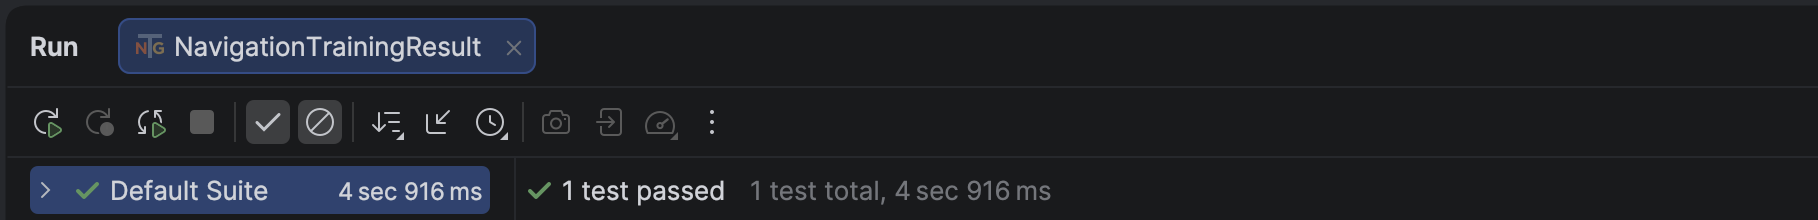
\includegraphics[width=0.8\textwidth]{pics/part2-result1.png}
	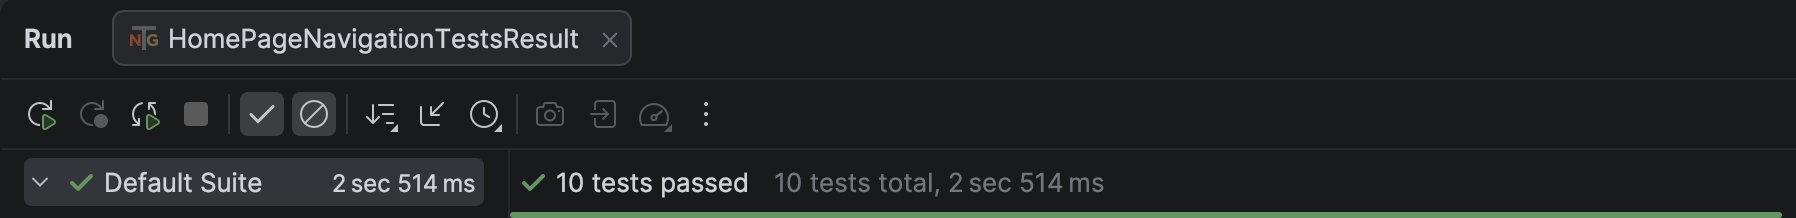
\includegraphics[width=0.8\textwidth]{pics/part2-result2.png}
	\caption{Результаты тестирования}
	\label{fig:results2}
\end{figure}

\pagebreak

\section*{Заключение}
\addcontentsline{toc}{section}{Заключение}

В ходе выполнения лабораторной работы были изучены и применены на практике основные инструменты автоматизированного тестирования программного обеспечения: фреймворк JUnit для модульного тестирования и Selenium WebDriver с TestNG для UI-тестирования веб-приложений.
В рамках первой задачи было проведено модульное тестирование библиотеки \texttt{lab-1.0.jar}. Для четырёх методов класса \texttt{DateUtils} (\texttt{isLeapYear}, \texttt{getDaysInMonth}, \texttt{daysBetween}, \texttt{isValidDate}) были разработаны тестовые сценарии с использованием классов эквивалентности и граничных значений. Всего было написано 54 теста. В результате тестирования выявлен следующий дефект: метод \texttt{getDaysInMonth} некорректно обрабатывает февраль високосного года, всегда возвращая 28 дней вместо 29. Методы \texttt{isLeapYear}, \texttt{daysBetween} и \texttt{isValidDate} отработали корректно. Таким образом, основная проблема библиотеки связана с недостаточной обработкой граничных условий при работе с високосными годами.
Во второй задаче было проведено UI-тестирование веб-сайта с использованием Selenium WebDriver и TestNG. Был реализован класс \texttt{DriverSetup} для инициализации браузера и авторизации, а также два тестовых класса: \texttt{NavigationTrainingResult}, проверяющий навигацию до страницы "Support" и структуру формы на ней, и \texttt{HomePageNavigationTestsResult}, выполняющий комплексную проверку главной страницы (заголовок, верхнее меню, пользовательская информация, логотип, футер, адаптивные классы). Все тесты были успешно пройдены.
В результате выполнения работы были получены практические навыки:
\begin{itemize}
\item создания модульных тестов с использованием фреймворка JUnit 5;
\item применения параметризованных тестов с аннотациями \texttt{@ParameterizedTest} и \texttt{@ValueSource};
\item использования методов подготовки и завершения тестов (\texttt{@BeforeEach}, \texttt{@AfterEach});
\item разработки UI-тестов с помощью Selenium WebDriver;
\item организации тестирования с использованием фреймворка TestNG;
\item реализации паттерна Page Object для структурирования тестового кода;
\item настройки конфигурации тестов через файл \texttt{suite.xml}.
\end{itemize}
Автоматизированное тестирование позволило эффективно выявить дефекты в тестируемой библиотеке и подтвердить корректность работы веб-приложения, что демонстрирует важность и практическую значимость применения автоматизированных инструментов тестирования в процессе разработки программного обеспечения.

\pagebreak

\begin{thebibliography}{3}
	\bibitem{[1]} Гпенфорд Майерс, Том Баджетг, Кори Сандлер <<Искусство тестирования программ, 3-е издание>>, Диалектика, 2012, 272 с.
\end{thebibliography}

\pagebreak

\section*{Приложение 1. Исходный код DateUtilsTest}

\begin{lstlisting}
import org.junit.jupiter.api.AfterEach;
import org.junit.jupiter.api.BeforeEach;
import org.junit.jupiter.params.ParameterizedTest;
import org.junit.jupiter.params.provider.ValueSource;
import org.junit.jupiter.api.Test;
import ru.spbstu.hsai.DateUtils;

import static org.junit.jupiter.api.Assertions.*;

public class DateUtilsTest {

    private long startTime;
    private String testDescription;

    @BeforeEach
    public void setUp() {
        startTime = System.currentTimeMillis();
        testDescription = "Running test";
        System.out.println("=== Setup: Test environment initialized ===");
    }

    @AfterEach
    public void tearDown() {
        long duration = System.currentTimeMillis() - startTime;
        System.out.println("=== Teardown: Test completed in " + duration + "ms ===\n");
    }

    // ==================== ТЕСТЫ ДЛЯ isLeapYear ====================

    @ParameterizedTest
    @ValueSource(ints = {2000, 2004, 2020, 2024, 2400})
    public void testIsLeapYear_ValidLeapYears(int year) {
        boolean result = DateUtils.isLeapYear(year);
        assertTrue(result, "Год " + year + " должен быть високосным");
    }

    @ParameterizedTest
    @ValueSource(ints = {1900, 2001, 2019, 2023, 2100})
    public void testIsLeapYear_ValidNonLeapYears(int year) {
        boolean result = DateUtils.isLeapYear(year);
        assertFalse(result, "Год " + year + " не должен быть високосным");
    }

    @ParameterizedTest
    @ValueSource(ints = {0, -1, -100})
    public void testIsLeapYear_InvalidYears(int year) {
        assertThrows(IllegalArgumentException.class, () -> {
            DateUtils.isLeapYear(year);
        }, "Год " + year + " должен выбрасывать IllegalArgumentException");
    }

    // ==================== ТЕСТЫ ДЛЯ getDaysInMonth ====================

    @ParameterizedTest
    @ValueSource(ints = {1, 3, 5, 7, 8, 10, 12})
    public void testGetDaysInMonth_31DaysMonths(int month) {
        int days = DateUtils.getDaysInMonth(2023, month);
        assertEquals(31, days, "Месяц " + month + " должен иметь 31 день");
    }

    @ParameterizedTest
    @ValueSource(ints = {4, 6, 9, 11})
    public void testGetDaysInMonth_30DaysMonths(int month) {
        int days = DateUtils.getDaysInMonth(2023, month);
        assertEquals(30, days, "Месяц " + month + " должен иметь 30 дней");
    }

    @ParameterizedTest
    @ValueSource(ints = {2023, 2019, 1900})
    public void testGetDaysInMonth_FebruaryNonLeapYear(int year) {
        int days = DateUtils.getDaysInMonth(year, 2);
        assertEquals(28, days, "Февраль " + year + " должен иметь 28 дней");
    }

    @ParameterizedTest
    @ValueSource(ints = {2020, 2024, 2000})
    public void testGetDaysInMonth_FebruaryLeapYear(int year) {
        int days = DateUtils.getDaysInMonth(year, 2);
        assertEquals(29, days, "Февраль " + year + " возвращает 28 дней");
    }

    // ==================== ТЕСТЫ ДЛЯ daysBetween ====================

    @ParameterizedTest
    @ValueSource(strings = {
            "2023-01-01",
            "2023-06-15",
            "2023-12-31",
            "2024-02-29"
    })
    public void testDaysBetween_SameDates(String date) {
        int days = DateUtils.daysBetween(date, date);
        assertEquals(0, days, "Разница между одинаковыми датами должна быть 0");
    }

    @ParameterizedTest
    @ValueSource(strings = {
            "2023-01-01,2023-01-10",
            "2023-03-01,2023-03-15",
            "2023-12-01,2023-12-31"
    })
    public void testDaysBetween_ConsecutiveDates(String dates) {
        String[] parts = dates.split(",");
        int days = DateUtils.daysBetween(parts[0], parts[1]);
        assertTrue(days > 0, "Разница должна быть положительной");
    }

    @Test
    public void testDaysBetween_AbsoluteValue() {
        int days1 = DateUtils.daysBetween("2023-01-01", "2023-01-10");
        int days2 = DateUtils.daysBetween("2023-01-10", "2023-01-01");
        assertEquals(days1, days2, "Разница должна быть абсолютным значением");
        assertEquals(9, days1);
    }

    // ==================== ТЕСТЫ ДЛЯ isValidDate ====================

    @ParameterizedTest
    @ValueSource(strings = {
            "2023-01-01",
            "2023-12-31",
            "2024-02-29",
            "2000-01-01",
            "2023-06-15"
    })
    public void testIsValidDate_ValidDates(String date) {
        boolean result = DateUtils.isValidDate(date);
        assertTrue(result, "Дата " + date + " должна быть валидной");
    }

    @ParameterizedTest
    @ValueSource(strings = {
            "2023-13-01",    // неверный месяц
            "2023-00-01",    // нулевой месяц
            "2023-01-00",    // нулевой день
            "2023-01-32",    // день > 31
            "invalid",       // не формат
            "01-01-2023",    // неверный порядок
            "2023/01/01",    // неверный разделитель
            "2023.01.01",    // неверный разделитель
            "",              // пустая строка
            "2023-1-1",      // отсутствие ведущих нулей
            "23-01-01"       // короткий год
    })
    public void testIsValidDate_InvalidDates(String date) {
        boolean result = DateUtils.isValidDate(date);
        assertFalse(result, "Дата " + date + " должна быть невалидной");
    }
}
\end{lstlisting}

\pagebreak

\section*{Приложение 2. Исходный код DriverSetup}

\begin{lstlisting}
package ru.spbstu.hsai;

import org.openqa.selenium.By;
import org.openqa.selenium.WebDriver;
import org.openqa.selenium.chrome.ChromeDriver;
import org.testng.annotations.AfterTest;
import org.testng.annotations.BeforeTest;

public class DriverSetup {

    // Общий экземпляр драйвера для всех тестовых классов пакета
    protected static WebDriver driver;

    // Выполняется один раз перед всеми тестами в suite
    // Требование TestNG: метод должен быть public static
    @BeforeTest
    public static void setup() {
        // Запуск браузера (Selenium Manager сам скачает драйвер)
        driver = new ChromeDriver();

        // 1. Open test site by URL
        driver.navigate().to("https://jdi-testing.github.io/jdi-light/index.html");

        // 3. Perform login
        driver.findElement(By.cssSelector("html > body > header > div > nav > ul.uui-navigation.navbar-nav.navbar-right > li > a > span")).click();
        driver.findElement(By.id("name")).sendKeys("Roman");
        driver.findElement(By.id("password")).sendKeys("Jdi1234");
        driver.findElement(By.id("login-button")).click();
    }

    // Выполняется после всех тестов: освобождение ресурсов
    // Требование TestNG: метод должен быть public static
    @AfterTest
    public static void exit() {
        //10. Close Browser
        driver.close();
    }
}
\end{lstlisting}

\pagebreak

\section*{Приложение 3. Исходный код \\NavigationTrainingResult}

\begin{lstlisting}
package ru.spbstu.hsai;

import org.openqa.selenium.By;
import org.openqa.selenium.JavascriptExecutor;
import org.openqa.selenium.OutputType;
import org.openqa.selenium.TakesScreenshot;
import org.openqa.selenium.WebElement;
import org.openqa.selenium.support.ui.ExpectedConditions;
import org.openqa.selenium.support.ui.WebDriverWait;
import org.testng.annotations.Test;
import org.testng.asserts.SoftAssert;

import java.io.File;
import java.io.FileWriter;
import java.io.IOException;
import java.time.Duration;
import java.util.List;

public class NavigationTrainingResult extends DriverSetup {

    private void navigateToSupport() {
        WebDriverWait wait = new WebDriverWait(driver, Duration.ofSeconds(15));

        try {
            // Открыть подменю "Service"
            WebElement serviceMenu = wait.until(ExpectedConditions.elementToBeClickable(
                    By.xpath("//a[contains(text(), 'Service')]")
            ));
            serviceMenu.click();
            Thread.sleep(500);

            // Кликнуть по пункту "Support" в выпавшем подменю
            WebElement supportLink = wait.until(ExpectedConditions.elementToBeClickable(
                    By.xpath("//a[contains(text(), 'Support')]")
            ));
            supportLink.click();
            Thread.sleep(1500);

        } catch (Exception e) {
            throw new RuntimeException("Не удалось перейти на страницу Support", e);
        }
    }

    // Сохранение скриншота и HTML при падении теста для отладки
    private void saveDebugInfo(String testName, Exception e) {
        try {
            File src = ((TakesScreenshot) driver).getScreenshotAs(OutputType.FILE);
            src.renameTo(new File("error_" + testName + ".png"));

            String html = driver.getPageSource();
            FileWriter writer = new FileWriter("error_" + testName + ".html");
            writer.write(html);
            writer.close();

            System.out.println("DEBUG: Скриншот и HTML сохранены для теста " + testName);
        } catch (IOException ex) {
            ex.printStackTrace();
        }
    }

    @Test
    public void testSupportPageFullCheck() {
        SoftAssert softAssert = new SoftAssert();
        String testName = "SupportPage";

        try {
            // 1. Navigate to the "Support" page using the main menu navigation
            navigateToSupport();

            // 2. Assert that the page title contains the word "support" (case-insensitive)
            String title = driver.getTitle().toLowerCase();
            softAssert.assertTrue(
                    title.contains("support"),
                    "Page title should contain 'support'. Actual title: " + title
            );

            // 3. Assert that a form or contact block is present on the page
            List<WebElement> forms = driver.findElements(By.tagName("form"));
            softAssert.assertFalse(forms.isEmpty(), "Form or contact block should be present on the page");

            if (!forms.isEmpty()) {
                WebElement form = forms.get(0);

                // 4. Assert that the form is NOT displayed and visible to the user
                ((JavascriptExecutor) driver).executeScript("arguments[0].scrollIntoView(true);", form);
                Thread.sleep(500);
                softAssert.assertFalse(
                        form.isDisplayed(),
                        "Form should NOT be displayed and visible to the user"
                );

                // 5. Assert that the form contains at least one input field (<input>)
    
                List<WebElement> inputs = form.findElements(By.xpath(
                        ".//input[not(@type='hidden') and not(@type='submit') and not(@type='button')]"
                ));
                softAssert.assertTrue(
                        inputs.size() >= 1,
                        "Form should contain at least one input field. Found: " + inputs.size()
                );

                // 6. Assert that the form does NOT contain a textarea element
                List<WebElement> textAreas = form.findElements(By.tagName("textarea"));
                softAssert.assertTrue(
                        textAreas.isEmpty(),
                        "Form should NOT contain textarea element. But found: " + textAreas.size()
                );

                // 7. Assert that the form contains a submit button
                // Login-форма содержит <button> без атрибута type
                List<WebElement> submitButtons = form.findElements(By.xpath(
                        ".//button[@type='submit'] | .//input[@type='submit'] | .//button[not(@type)]"
                ));
                softAssert.assertTrue(
                        !submitButtons.isEmpty(),
                        "Form should contain a submit button. Found: " + submitButtons.size()
                );
            }

        } catch (Exception e) {
            saveDebugInfo(testName, e);
            softAssert.fail("Error in test " + testName + ": " + e.getMessage());
        }

        softAssert.assertAll();
    }
}
\end{lstlisting}

\pagebreak

\section*{Приложение 4. Исходный код \\HomePageNavigationTestsResult}

\begin{lstlisting}
package ru.spbstu.hsai;

import org.openqa.selenium.By;
import org.openqa.selenium.WebElement;
import org.testng.annotations.Test;
import java.util.List;
import static org.testng.Assert.*;

public class HomePageNavigationTestsResult extends DriverSetup {

    // 1. Проверка заголовка страницы
    @Test(priority = 1)
    public void testPageTitle() {
        String title = driver.getTitle();
        assertEquals(title, "Home Page",
                "Заголовок вкладки не совпадает с ожидаемым 'Home Page'. Получено: " + title);

        // Дополнительная проверка: заголовок не должен быть пустым
        assertFalse(title.trim().isEmpty(), "Заголовок страницы пустой");

        // Проверка, что заголовок содержит ключевое слово
        assertTrue(title.toLowerCase().contains("home"),
                "Заголовок должен содержать слово 'home'");
    }

    // 2. Проверка количества пунктов в верхнем меню
    @Test(priority = 3)
    public void testHeaderMenuCount() {
        List<WebElement> menuItems = driver.findElements(By.cssSelector("ul.uui-navigation.nav > li"));
        assertEquals(menuItems.size(), 4,
                "Количество пунктов в верхнем меню должно быть 4. Найдено: " + menuItems.size());
    }

    // 3. Проверка текстов пунктов верхнего меню
    @Test(priority = 4, dependsOnMethods = "testHeaderMenuCount")
    public void testHeaderMenuTexts() {
        List<WebElement> menuItems = driver.findElements(By.cssSelector("ul.uui-navigation.nav > li"));
        String[] expectedTexts = {"HOME", "CONTACT FORM", "SERVICE", "METALS & COLORS"};

        assertEquals(menuItems.size(), expectedTexts.length,
                "Количество элементов меню не совпадает с количеством ожидаемых текстов");

        for (int i = 0; i < expectedTexts.length; i++) {
            String actualText = menuItems.get(i).getText().trim().toUpperCase();
            assertEquals(actualText, expectedTexts[i],
                    "Текст пункта меню #" + (i+1) + " неверен. Ожидалось: '" + expectedTexts[i] +
                            "', получено: '" + actualText + "'");
        }
    }

    // 4. Проверка ссылок верхнего меню (href атрибуты)
    @Test(priority = 5, dependsOnMethods = "testHeaderMenuTexts")
    public void testHeaderMenuLinks() {
        List<WebElement> menuLinks = driver.findElements(By.cssSelector("ul.uui-navigation.nav > li > a"));

        assertEquals(menuLinks.size(), 4, "В верхнем меню должно быть 4 ссылки");

        String[] expectedHrefs = {"index.html", "contact.html", "service.html", "metals.html"};

        for (int i = 0; i < menuLinks.size(); i++) {
            WebElement link = menuLinks.get(i);
            String href = link.getAttribute("href");

            // Проверка, что ссылка отображается и кликабельна
            assertTrue(link.isDisplayed(), "Ссылка меню #" + (i+1) + " не отображается");
            assertTrue(link.isEnabled(), "Ссылка меню #" + (i+1) + " не активна");

            if (href != null && !href.trim().isEmpty()) {
                boolean containsExpected = false;
                for (String expected : expectedHrefs) {
                    if (href.toLowerCase().contains(expected.toLowerCase())) {
                        containsExpected = true;
                        break;
                    }
                }
                assertTrue(containsExpected || href.endsWith("#") || href.contains("jdi-testing"),
                        "href пункта меню #" + (i+1) + " должен содержать один из ожидаемых паттернов: " +
                                String.join(", ", expectedHrefs) + ". Получено: " + href);
            }
        }
    }

    // 5. Проверка кликабельности пунктов меню
    @Test(priority = 6, dependsOnMethods = "testHeaderMenuLinks")
    public void testHeaderMenuClickable() {
        List<WebElement> menuItems = driver.findElements(By.cssSelector("ul.uui-navigation.nav > li > a"));

        for (int i = 0; i < menuItems.size(); i++) {
            WebElement item = menuItems.get(i);

            // Проверка, что элемент отображается и активен (основная проверка кликабельности)
            assertTrue(item.isDisplayed(), "Пункт меню #" + (i+1) + " не отображается");
            assertTrue(item.isEnabled(), "Пункт меню #" + (i+1) + " не активен");
        }
    }

    // 6. Проверка имени залогиненного пользователя
    @Test(priority = 7)
    public void testLoggedInUserName() {
        WebElement userNameElement = driver.findElement(By.id("user-name"));
        assertTrue(userNameElement.isDisplayed(), "Элемент с именем пользователя не найден");

        String userName = userNameElement.getText().trim();
        assertFalse(userName.isEmpty(), "Имя пользователя пустое");

        // Проверка формата имени (должно содержать имя и фамилию)
        assertTrue(userName.toUpperCase().contains("ROMAN") || userName.toUpperCase().contains("IOVLEV"),
                "Неверное имя пользователя: " + userName + ". Ожидалось содержание 'ROMAN' или 'IOVLEV'");

        // Проверка, что имя не содержит специальных символов (кроме пробелов)
        assertTrue(userName.matches("^[a-zA-Z\\s]+$"),
                "Имя пользователя содержит недопустимые символы: " + userName);
    }

    // 7. Проверка аватара/иконки пользователя
    @Test(priority = 8, dependsOnMethods = "testLoggedInUserName")
    public void testUserAvatar() {
        WebElement userIcon = driver.findElement(By.cssSelector(".profile-photo, .user-icon"));

        // Основная проверка: элемент существует и видим
        assertTrue(userIcon.isDisplayed(), "Иконка пользователя не отображается");
        assertTrue(userIcon.isEnabled(), "Иконка пользователя не активна");

        // Проверяем, что элемент имеет размеры (не пустой)
        int width = userIcon.getSize().getWidth();
        int height = userIcon.getSize().getHeight();
        assertTrue(width > 0 && height > 0,
                "Иконка пользователя имеет нулевые размеры: " + width + "x" + height);

        String tagName = userIcon.getTagName();
        String innerText = userIcon.getText().trim();
        String className = userIcon.getAttribute("class");

        // Либо есть текст, либо класс содержит "icon"/"avatar"/"photo", либо это img/svg
        boolean hasVisualContent =
                !innerText.isEmpty() ||
                        className.toLowerCase().matches(".*(icon|avatar|photo|user).*") ||
                        tagName.equals("img") || tagName.equals("svg");

        assertTrue(hasVisualContent,
                "Элемент иконки пользователя не содержит визуального контента: tag=" + tagName +
                        ", class=" + className + ", text='" + innerText + "'");
    }
    // 8. Проверка логотипа сайта
    @Test(priority = 10)
    public void testSiteLogo() {
        // Поиск логотипа по различным селекторам
        WebElement logo = null;
        try {
            logo = driver.findElement(By.cssSelector(".brand-logo, .logo, img[alt*='logo'], .jdi-logo"));
        } catch (Exception e) {
            // Если не нашли по классам, ищем первый img в header
            logo = driver.findElement(By.cssSelector("header img"));
        }

        assertNotNull(logo, "Логотип сайта не найден");
        assertTrue(logo.isDisplayed(), "Логотип не отображается");

        // Проверка alt атрибута
        String alt = logo.getAttribute("alt");
        assertNotNull(alt, "У логотипа отсутствует атрибут alt");

        // Проверка кликабельности логотипа (должен вести на главную)
        WebElement logoLink = logo.findElement(By.xpath("./ancestor::a[1]"));
        assertNotNull(logoLink, "Логотип не обернут в ссылку");

        String href = logoLink.getAttribute("href");
        assertNotNull(href, "У ссылки логотипа отсутствует href");
        assertTrue(href.contains("index") || href.endsWith("/") || href.contains("jdi-testing"),
                "Логотип должен вести на главную страницу");
    }

    // 9. Проверка футера страницы
    @Test(priority = 11)
    public void testFooterContent() {
        // Проверяем наличие футера (не обязательно тега <footer>, может быть div/class)
        WebElement footer = driver.findElement(By.cssSelector("footer, .footer, [role='contentinfo']"));
        assertTrue(footer.isDisplayed(), "Футер страницы не отображается");

        // Проверка, что футер содержит какой-либо текст
        String footerText = footer.getText().trim();
        assertFalse(footerText.isEmpty(), "Текст футера пустой");

        // Опциональная проверка: футер должен содержать хотя бы одно из ожидаемых слов
        // (если структура сайта изменится, тест не упадёт критично)
        boolean hasExpectedContent =
                footerText.toLowerCase().contains("o") ||
                        footerText.toLowerCase().contains("copyright") ||
                        footerText.matches(".*\\d{4}.*") ||
                        footerText.toLowerCase().contains("jdi") ||
                        footerText.toLowerCase().contains("epam");

        assertTrue(hasExpectedContent,
                "Футер не содержит ожидаемого контента. Текст: '" + footerText + "'");
    }

    // 10. Проверка responsive элементов (наличие классов адаптивности)
    @Test(priority = 12)
    public void testResponsiveClasses() {
        // Проверка наличия container или wrapper классов
        WebElement mainContainer = driver.findElement(By.cssSelector(".container, .wrapper, .main-content"));
        assertNotNull(mainContainer, "Отсутствует основной контейнер страницы");

        // Проверка, что элементы имеют классы для адаптивности
        String containerClass = mainContainer.getAttribute("class");
        assertTrue(containerClass.contains("container") ||
                        containerClass.contains("wrapper") ||
                        containerClass.contains("content"),
                "Основной контейнер должен иметь класс container/wrapper/content");
    }
}
\end{lstlisting}

\end{document}